\subsection{Independent Agent}\label{Independent_Agent}
The independent agent is implemented with no message sharing. In this implementation, each unit is controlled by itself only, so the decisions are made based only on the knowledge available to that particular unit. 


%decision by one unit = decision other unit. this may inclue friendly firing

%Due to combining partial knowledge from its units, the cooperative agent performs better than the independent agent. This scenario can be explained with figure-~\ref{fig:coop_vs_ind}. Here we consider a $3$ by $3$  board where the visible square is $1$ and the black circled units are controlled by the cooperative agent. Now unit-2 can move to the middle cell of top row, so that if unit-1 is killed by enemy unit-A then unit-2 can attack it in the next turn. The independent team has no such message passing, so unit-2 will choose its action without considering the effect on its team score. Therefore the performance of the independent agent is not as good as the cooperative agent.
%and then unit-2 will move to the middle cell of top row, so that if unit-1 is killed by enemy unit-A then unit-2 can attack it in the next turn. But independent team has no such message passing. So unit-2 will choose is action with out considering the effect on team score. Therefor the performance of independent agent is not as good as the cooperative agent.


%\begin{figure}[htb]

%\begin{minipage}[b]{1.0\linewidth}
%  \centering
%  \centerline{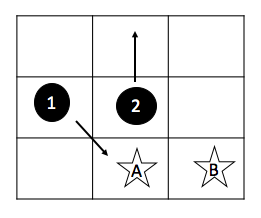
\includegraphics[width=3.5cm]{coop_vs_ind}}
%  \vspace{2.0cm}
  
%\end{minipage}
%\caption{Comparing movements of independent agent with cooperative agent}
%\label{fig:coop_vs_ind}
%
%\end{figure}

%\vspace{-.5 cm}